% !TEX root = ../thesis.tex


\chapter{Conclusion and Future Work}
We investigated the possibility of evaporative cooling in a box potential which gets dynamically compressed over time. In a static box potential, efficient evaporative cooling is not easily possible due to decreasing densities. We studied an optical box potential made out of two ring beams where we reduce the ring diameter to compress the trap. A numerical simulation of the gas dynamics during evaporation was performed for $^{87}$Rb using different initial phase space densities and atom numbers. We found that efficient evaporation is indeed possible in such a trap. However, one important requirement for this is a high initial phase space density as otherwise only a small fraction of the initial atoms can be captured.
One possibility to achieve such a high initial phase space density would be through several cycles of gray molasses cooling with compression stages in between. During gray molasses cooling, the gas can expand freely which is why its density decreases under normal conditions. In a box trap however, the trapping potential can remain active during the gray molasses, allowing for longer durations and therefore lower temperatures. Intermittent compression could then increase the phase space density even further to achieve the best possible starting conditions for evaporation.

A similar scheme could also be employed for other atomic species, e.g.\ $^{39}$K. Its broad Feshbach resonance can be used to control the scattering length \cite{k39Feshbach} and at similar scattering length, its lower mass would lead to higher elastic collision rates, theoretically increasing the evaporation efficiency.

In our simulated cases, we found that long evaporation times were necessary to achieve high phase space densities. This may partly be due to still poor optimisation.
Firstly, optimisation of the evaporation trajectories has to be done manually so far as the inherent statistical scatter of the numerical approach prevents non-linear optimisation strategies. Secondly, one simulation run can take between 7 and 10 minutes on a high-end desktop processor\footnote{AMD Ryzen 7 3700X} which makes brute-force optimisation difficult for a larger set of independent variables. This time constraint was one of the deciding reasons why only one ramp step was employed. It is expected that a subdivision in multiple steps could greatly benefit the evaporation by providing more finely grained control over the density.

Real experiments have also shown that the use of machine learning for optimisation can lead to drastic improvements both in atom numbers and evaporation times \cite{machinelearning1,machinelearning2}. It also brings the benefit that not a full search of the entire parameter space is necessary. It is thus possible that a better optimised evaporation trajectory could be developed by discretising the ramp into several steps and then using a machine learning procedure to find the best combination.

Lastly, we also want to give a brief outlook on how a beam like the one we used in the simulation can be created. Hueck et al \cite{axiconSM} have demonstrated the creation of sharp ring shaped beams with variable diameter between \SI{50}{\micro\meter} and \SI{200}{\micro\meter} in 2017 by using multiple axicon \cite{McLeod} lenses and larger rings with a radius of \SI{400}{\micro\meter} are also possible \cite{MANEK199867}.
The setup designed by Hueck is shown in Figure~\ref{fig:proposed_beam}.
\begin{figure}[htbp]
    \centering
    \begin{tikzpicture}
    \node[anchor = south west, inner sep=0] (Image) at (0,0) {\includegraphics[page=2,trim=160 590 55 70,clip]{Evap/AxiconSetup/File}};
    \begin{scope} [x={(Image.south east)},y={(Image.north west)}]
        \node[rectangle, rounded corners,draw=none,inner sep=1pt] at (0.225,0.152) {$f=\SI{400}{mm}$};
        \node[rectangle, rounded corners,draw=none,inner sep=1pt] at (0.922,0.152) {\parbox{1.5cm}{\centering Image Plane}};
        \node[rectangle, rounded corners,draw=none,inner sep=1pt] at (0.074,0.89) {$\SI{10}{\degree}$ Axicon};
        \node[rectangle, rounded corners,draw=none,inner sep=1pt] at (0.27,0.89) {$\SI{10}{\degree}$ Axicon};
        \node[rectangle, rounded corners,draw=none,inner sep=1pt] at (0.8,0.89) {Movable $\SI{2}{\degree}$ Axicon};
    \end{scope}
\end{tikzpicture}
    \caption[Optical setup to create a ring beam with dynamically adjustable radius]{Adapted from \cite{axiconSM}. Optical setup to create a ring beam with dynamically adjustable radius. Not shown here is an additional microscope that demagnifies the beam from the image plane to the target plane.}
    \label{fig:proposed_beam}
\end{figure}
Here, the first axicon creates a ring shaped beam which is then optically inverted by the second axicon. This is done to shift the steep edge to the inner side. The third axicon collimates the beam and by moving it along the optical axis, different diameters can be achieved. After this, a high-resolution microscope can be used to demagnify the ring and project it onto the atomic cloud.
The use of a motorised translation stage would then provide precise dynamic control over the diameter.

An axicon ring could also be used in conjunction with a DMD to produce even steeper walls if the beam is not already diffraction limited. This would retain a larger intensity than the use of a DMD alone to shape a ring potential.


% \vspace{1ex}\noindent
% The simulation program is publicly available and can be used for future experiments with different potential geometries as well. 
% Arbitrary potentials can be implemented through the use of a simple API, as long as they fulfill the requirement of axial symmetry in $x$ and $y$ direction for the doubling procedure.